\begin{figure*}\centering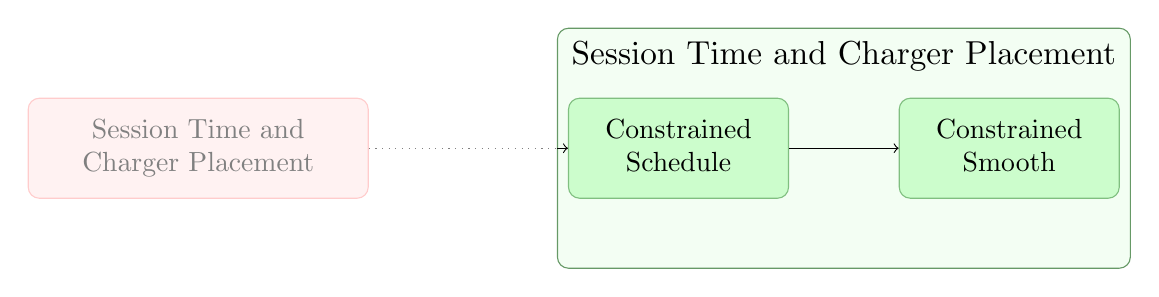
\begin{tikzpicture}
\node[rectangle, draw=gray!80!green, fill=gray!10!green!5, minimum width=\textwidth*0.6, minimum height=1.2in, rounded corners, label={[label distance=-0.67cm]above:\scalebox{1.2}{Session Time and Charger Placement}}](outline) at (0,0){};
	\node[rectangle, draw=green!50!black!50, fill=black!3!green!20, minimum width=1.1in, minimum height=0.5in, rounded corners](problem1) at (-2.1,0) {\begin{tabular}{c} Constrained \\ Schedule\end{tabular}}; 
	\node[rectangle, draw=green!50!black!50, fill=black!3!green!20, minimum width=1.1in, minimum height=0.5in, rounded corners](problem3) at (2.1,0) {\begin{tabular}{c}Constrained \\ Smooth\end{tabular}}; 
	\node[rectangle, draw=red!20, fill=red!5, text=black!50, minimum width=1.7in, minimum height=0.5in, rounded corners](problem0) at (-8.2,0){\begin{tabular}{c}Session Time and \\ Charger Placement\end{tabular}};
	\draw[draw=black!50, dotted] (problem0.east) -- (outline.west);
	\draw[->] (outline.west) -- (problem1.west);
	\draw[->, draw=black] (problem1.east) -- (problem3.west);
\end{tikzpicture}\caption{Processing chain for the Final Optimization set} \label{fig:set3Chain}\end{figure*}

